% chktex-file 2% chktex-file 29
% chktex-file 13
\documentclass{report}
\usepackage{setspace}
\usepackage[a4paper, total={7in, 9in}]{geometry}
\usepackage[fleqn]{amsmath}
\usepackage{empheq}
\usepackage{amssymb}
\usepackage{amsthm}
\usepackage{gensymb}
\usepackage[fleqn]{cases}
\usepackage{multicol}
\usepackage{color}
\usepackage{stix}
\usepackage{chngcntr}
\usepackage{tikz}
\usepackage{enumitem}
\usepackage{pgfplots}
\usepackage{etoolbox}
\usetikzlibrary{calc,matrix,arrows}
\usetikzlibrary{decorations.pathmorphing,patterns}

\counterwithout{equation}{chapter}
\setlength{\columnseprule}{1pt}
\setlength{\columnsep}{24pt}
\setcounter{chapter}{14}
\hfuzz=100pt

\newcommand{\pgfplotsdrawaxis}{\pgfplots@draw@axis}
\makeatother
\pgfplotsset{only axis on top/.style={axis on top=false, after end axis/.code={
                    \pgfplotsset{axis line style=opaque, ticklabel style=opaque, tick style={thick,opaque},
                        grid=none}\pgfplotsdrawaxis}}}

\newtheorem{theorem}{Theorem}

\begin{document}

\newcommand{\sol}[1]{

    \noindent \textbf{Sol.}
}
\newcommand{\prooff}[1]{

    \noindent \textbf{Proof.}
}
\newcommand\m[1]{\begin{pmatrix}#1\end{pmatrix}}
\newcommand\vm[1]{\begin{vmatrix}#1\end{vmatrix}}
\newenvironment{amatrix}[1]{%
    \left(\begin{array}{@{}*{#1}{c}|c@{}}
        }{%
    \end{array}\right)
}
\newenvironment{cequation}{
    \makeatletter
    \setbool{@fleqn}{false}
    \makeatother
    \begin{equation*}
        }{\end{equation*}}

\begin{titlepage}
    \raggedleft{}
    \rule{1pt}{\textheight}
    \hspace{0.02\textwidth}
    \parbox[b]{0.75\textwidth}{

    {\Huge\bfseries Solution Book of \\[0.5\baselineskip] Mathematic}\\[2\baselineskip]
    {\large\textit{Ssnior 2 Part I}}\\[4\baselineskip]
    {\Large\textsc{MELVIN CHIA}}

    \vspace{0.5\textheight}

    {\noindent Written on 9 October 2022}\\[\baselineskip]
    }

\end{titlepage}

\doublespacing{}
\tableofcontents
\singlespacing{}
\newpage

\begin{multicols}{2}

    \chapter{Circle}

    \section{Standard Equation of a Circle}

    The circle is a locus of points in a plane that are equidistant from a fixed
    point called the centre of the circle. The distance between the centre and the
    points on the circle is called the radius of the circle.

    \begin{center}
        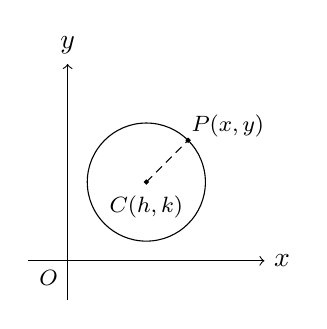
\begin{tikzpicture}[scale=0.5]
            \draw[->] (-1,0) -- (5,0) node[right] {$x$};
            \draw[->] (0,-1) -- (0,5) node[above] {$y$};
            \draw (2,2) circle (1.5);
            \filldraw[black] (2,2) circle (0.05);
            \draw[black] (2,1.9) node[below] {\footnotesize$C(h,k)$};
            \filldraw[black] (3.061, 3.061) circle (0.05);
            \draw[black] (2.9, 2.9) node[above right] {\footnotesize$P(x,y)$};
            \draw[black, densely dashed] (2,2) -- (3.061, 3.061);
            \draw[black] (0,0) node[below left] {\footnotesize$O$};
        \end{tikzpicture}
    \end{center}

    The standard equation of a circle is given by
    \begin{cequation}
        (x-h)^2+(y-k)^2=r^2
    \end{cequation}
    where $(h,k)$ is the centre of the circle and $r$ is the radius of the circle.

    If the centre of the circle is at the origin, then the equation of the circle
    is
    \begin{cequation}
        x^2+y^2=r^2\ \ \ \ \ (r>0)
    \end{cequation}

    \subsection{Practice 1}

    \begin{enumerate}
        \item Find the equation of the circle with centre $(3, -1)$ and radius $2$.
        \item Find the equation of the circle with centre $(-2, 9)$ and passing through the
              point $(1, 5)$.
    \end{enumerate}

    \subsection{Exercise 16.1}

    \begin{enumerate}
        \item Find the equation of the circle with centre at the origin and radius $7$.
        \item Find the equation of circle of each of the following description:
              \begin{enumerate}
                  \item Passing through the points $(5, -3)$ and centre at $(2, 1)$.
                  \item Centre at $(3, 2)$ and radius $4$.
                  \item Centre at $(a, b)$ and radius $a+b$.
              \end{enumerate}
        \item Given that the coordinates of two points on the end of the diameter of a circle
              are $(5, -3)$ and $(3, 1)$, find the equation of the circle.
        \item Find the equation of the circle with a diameter connected by the points $(-3,
                  4)$ and $(9, 2)$.
        \item Given two points $P(-2, 2)$ and $Q(4, 6)$, find the equation of the circle wuth
              line $PQ$ as its diameter.
        \item Turn the equation $x^2+y^2-6x+12y+41=0$ into the standard form, and find the
              centre and radius of the circle.
    \end{enumerate}

    \section{General Equation of a Circle}

    Expand the standard equation of a circle, we get
    \begin{cequation}
        x^2+y^2-2hx-2ky+h^2+k^2-r^2=0
    \end{cequation}
    \setlength{\belowdisplayskip}{0pt} \setlength{\belowdisplayshortskip}{0pt}
    \setlength{\abovedisplayskip}{0pt} \setlength{\abovedisplayshortskip}{0pt}
    Let $g=-h$, $f=-k$, $c=h^2+k^2-r^2$, we get the general equation of a circle
    \begin{cequation}
        x^2+y^2+2gx+2fy+c=0
    \end{cequation}
    \begin{flalign*}
        \text{From }c=h^2+k^2-r^2\text{, we have }r^2 & =h^2+k^2-c              & \\
        r                                             & =\sqrt{h^2+k^2-c}       & \\
                                                      & =\sqrt{(-g)^2+(-f)^2-c} & \\
                                                      & =\sqrt{g^2+f^2-c}
    \end{flalign*}
    \noindent Thus,
    \begin{enumerate}
        \item When $g^2+f^2-c>0$, the image is a real circle with centre $(g,f)$ and radius
              $\sqrt{g^2+f^2-c}$.
        \item When $g^2+f^2-c=0$, the image is point $(g,f)$.
        \item When $g^2+f^2-c<0$, the image does not exist.
    \end{enumerate}

    \subsection{Practice 2}

    \begin{enumerate}
        \item Find the centre and radius of the circle with equation $x^2+y^2-6x-8y+21=0$.
        \item Find the equaton of the circle that passes through the following points:
              \begin{enumerate}
                  \item $A(0, 0)$, $B(2, 0)$, $C(0, -3)$.
                  \item $K(0, 3)$, $L(1, 2)$, $M(2, -1)$.
              \end{enumerate}
        \item Given that the vertices of $\Delta ABC$ are $(1, 2)$, $(2, 5)$ and $(-1, 2)$,
              find the equation of the circumcircle of $\Delta ABC$.
    \end{enumerate}

    \subsection{Exercise 16.2}

    \begin{enumerate}
        \item Find the centre and radius of the circle with the following equation:
              \begin{enumerate}
                  \item $x^2+y^2-64=0$
                  \item $x^2+y^2-4x-8y=44$
                  \item $x^2+y^2-8x=0$
                  \item $9x^2+9y^2+2x-6y-6=0$
                  \item $9x^2+9y^2+2x-6y-6=0$
              \end{enumerate}
        \item Find the equation of the circle that passes through the following points:
              \begin{enumerate}
                  \item $A(1, 1)$, $B(1, -1)$, $C(-2, 1)$
                  \item $F(0, 0)$, $G(3, -3)$, $H(-1, 0)$
                  \item $P(1, 0)$, $Q(0, -3)$, $R(3, 4)$
              \end{enumerate}
        \item A circle passes through point $A(2, 2)$ and $B(5, 3)$ while intersecting the
              line $x+y=4$ at y-axis. Find the equation of the circle.
    \end{enumerate}

\end{multicols}
\end{document}